\documentclass[final]{beamer} % use beamer

%\usepackage[usenames,dvipsnames]{xcolor}
\usepackage[orientation=portrait,size=a0,scale=1.3]{beamerposter}
\usepackage[english]{babel}
\usepackage[utf8]{inputenc}
\usepackage{amsfonts}
\usepackage{amsthm}
\usepackage{amsmath}
\usepackage{enumerate}
\usepackage{pgf}
\usepackage{palatino}
\usepackage{comment}
\usepackage{natbib}
\usepackage{paralist}
\usepackage{epstopdf}
\usepackage{algorithm}
\usepackage{caption}
\usepackage{algorithmic}
\usepackage{tcolorbox}
\usepackage{multicol}
\setbeamertemplate{bibliography item}[text]

\setlength{\leftmargini}{2cm}


%\usetheme{bpiresicml2013}
\usepackage{beamerthemebpiresicml2013-p}

%\setbeamercolor{block title}{fg=black,bg=white}
%\setbeamercolor{block body}{fg=black,bg=white}
%--set colors for alerted blocks (with frame)----------------------------------
%--textcolor = fg, backgroundcolor = bg, dblue is the jacobs blue
%\setbeamercolor{block alerted title}{fg=white,bg=uofagreen!70}%frame color
 %\setbeamercolor{block alerted body}{fg=black,bg=uofagreen!10}%body color

%==Title, date and authors of the poster=======================================

\newcommand{\cA}{\mathcal{A}}
\newcommand{\cB}{\mathcal{B}}
\newcommand{\cL}{\mathcal{L}}
\newcommand{\cW}{\mathcal{W}}
\newcommand{\cF}{\mathcal{F}}
\newcommand{\lt}{\ell_t}
\newcommand{\bd}{\mathrm{bd}}
\newcommand{\R}{\mathbb{R}}
\newcommand{\bS}{\mathbb{S}}
\newcommand{\ind}{\mathbb{I}}
\newcommand{\hf}{\hat{f}}

\newcommand{\Exp}[1]{\mathbb{E}\left[ #1 \right]} 
\newcommand{\seto}[1]{\left\{#1\right\}}
\newcommand{\norm}[1]{\left\| #1 \right\|}
\newcommand{\ip}[1]{\langle#1\rangle}
\newcommand{\set}[2]{\left\{#1 \,:\, #2 \right\}}

\DeclareMathOperator*{\argmin}{argmin}
\DeclareMathOperator*{\argmax}{argmax}
%\newcommand{\bi}{\begin{itemize}
%\newcommand{\ei}{\end{itemize}}


\newtheorem{thm}{Theorem}[section]
%\addtobeamertemplate{block begin}{}{\setlength{\parskip}{35pt plus 1pt minus 1pt}}

\title{Following the Leader and Fast Rates in Linear Prediction: Curved Constraint Sets and Other Regularities}
\author{Ruitong Huang, Tor Lattimore, Andr\'as Gy\"orgy, Csaba Szepesv\'{a}ri}


\begin{document}

\begin{frame}[c]
	\vspace{-1.5cm}

	\begin{columns}[t,totalwidth=\textwidth]
	
	\begin{column}{0.01\textwidth}
	\end{column}
%------------------------------------------------------------------------------
% The first column
%------------------------------------------------------------------------------	

		
 	\begin{column}{.32\textwidth}% the right size for a 3-column layout
	
		\begin{block}{Background}
		\begin{minipage}{.9\linewidth}
			\setbeamercolor{block title}{fg=black, bg=uofagreen!10}
			\begin{block}{}
			\vspace{-3.5cm}
			{\centering \bf Online Learning Protocol\\}
			For each round $t$:
				\begin{itemize}
					\item  Learner predicts $w_t\in \cW$;
					\item  Adversary picks $\lt\in \cL$;
					\item  Learner suffers loss $\lt(w_t)$ and learns $\lt$.
				\end{itemize}
			\end{block}	
		\end{minipage}
			
		{\large \it Goal:} Minimizing the regret (in $n$ rounds):
		\[
		R_n = \sum_{t=1}^{n} \lt(w_t) - \min_{w\in\cW} \sum_{t=1}^{n} \lt(w).
		\]
		
		\vspace{1cm}
		{\large Fast rates in online convex optimization:}
		\begin{itemize}
			\item Curved loss functions: strongly convex, exp-concave  \citep{MF92,hazan2007logarithmic,bartlett2007adaptive,kakade2009mind,orabona2012beyond,vanerven2015fast}.
			\item Small loss of the optimal predictor  \citep{FrSc97}.
			\item Small variations of losses   \citep{RakhlinS13}.
		\end{itemize}
	
		\end{block}
		\begin{block}{Problem Setting}
		{\centering Linear Loss: $\lt(w) = \ip{f_t, w}$}.
		\begin{minipage}{.9\linewidth}
			\setbeamercolor{block title}{fg=black, bg=uofagreen!10}
			\begin{block}{}
				\vspace{-2cm}
		 		\begin{tcolorbox}[title filled,colbacktitle=uofagreen!5, coltitle = black, width = 0.9\textwidth, colback = uofagreen!10, colframe = red,arc = 16pt]
			 		Follow the leader (FTL):\\
			 		$\quad \quad \quad w_t = \argmin_{w\in \cW} \sum_{i=1}^{t-1} \ip{f_i,w}.$
		 		\end{tcolorbox}	
			 	\begin{itemize}
			 		\item Optimal in the stochastic setting;
			 		\item Proven to fail in the adversarial setting;
			 		\item Regularization helps, but suffers a slower learning rate $O(\sqrt{n})$.
			 	\end{itemize}
			\end{block}
		\end{minipage}

		 \vspace{1cm}
	 	{\large \alert{To what extent, FTL can still perform well?}}
	 	\vspace{1cm}
	 	\begin{tcolorbox}[title = \vspace{0.4cm}\textbf{\large Our contribution} \vspace{0.4cm}, title filled, width = 0.9\textwidth, colback = uofagreen!10, colframe = red, arc = 16pt]
	 		Curvature of $\cW$ helps FTL to achieve fast rate!
	 	\end{tcolorbox}
		\end{block}

	
		\begin{block}{FTL and the Support Function}
			Support function of $\cW$:
			\qquad $
			\Phi(\Theta) = \max_{w\in\cW} \ip{w, \Theta}.
			$
			\medskip
			
			Average negative loss:
			\qquad \quad$\displaystyle
			\Theta_t = -\frac1t \sum_{i=1}^t f_i.
			$
			
			\begin{minipage}{.9\linewidth}
				\setbeamercolor{block title}{fg=black, bg=uofagreen!10}
			\begin{alertblock}{Regret of FTL: }
				\vspace{-1cm}
				\[
				R_n = \sum_{t=1}^n t\,\ip{ w_{t+1}-w_t,\Theta_t} = \sum_{t=1}^{n} t\,D_{\Phi}(\Theta_t,\Theta_{t-1}).
				\]
				\begin{itemize}
					\item Bregman divergence: $D_{\Phi}(\theta', \theta) = \Phi(\theta') - \Phi(\theta) - \ip{ \nabla\Phi(\theta), \theta' - \theta}$.
					\item Shows implicit connection with stability.
					\item Shows implicit connection with curvature. 
				\end{itemize}
			\end{alertblock}
			\end{minipage}
		
		\end{block}

%\medskip

		\begin{block}{Intuition}
						%\vspace{-0.5cm}
						\begin{minipage}[b]{0.55\textwidth}
						\begin{itemize}
							\item $\cW = \set{w}{\|w\|_2\le 1}$;
							\item $f_t$ are i.i.d.;
							\item $\Exp{f_t} = \mu = (-1,0)$;
							\item $w^* = (1,0)$;
							\item $\ip{w^*,\mu} = -1$;
						\end{itemize}
						\end{minipage}
						\begin{minipage}[b]{0.37\textwidth}
						{\includegraphics[width=\textwidth, trim={6.2cm 6cm 2cm 0},clip]{figures/ExcessError}}
						\end{minipage}
					
						\begin{itemize}
							\item $E = \set{-\theta}{\|\theta - \mu\|_2 \le \epsilon}$, expect $-\mu_t \in E$ w.h.p. for $\epsilon=O(1/\sqrt{t})$;
							\item Excess loss for $\mu_t$ is $|\tilde{B}D| \le |BD| \le \epsilon^2 = O(1/t)$.
							\item Regret: $O(\log n)$
						\end{itemize}
				\end{block}


	\end{column}
%------------------------------------------------------------------------------
% The second column
%------------------------------------------------------------------------------	
	\begin{column}{0.01\textwidth}
	\end{column}
	
	\begin{column}{.32\textwidth}% the right size for a 3-column layout

		\begin{block}{Curved Constraint Sets}			
			\begin{minipage}{.9\linewidth}
			\vspace{-0.5cm}
			\setbeamercolor{block title}{fg=black, bg=uofagreen!10}
					\begin{block}{Principal Curvature}
						\vspace{-1.5cm}
						\begin{itemize}
						\item $\cW$ is $C^2$: the boundary $\bd(\cW)$ is a $C^2$ submanifold of $\R^d$;
						\item Gauss map: $u_{\cW} : \bd(\cW) \to \bS^{d-1}$  (unit sphere);
						%\begin{itemize}
						%	\item continuously differentiable normal unit vector field
						%\end{itemize}
						\item Principal curvatures: eigenvalues of  $\nabla u_{\cW}(p)$.
						\begin{itemize}
							\item eigenvalues of $\nabla^2 f(0)$ in the transformed coordinate system;
							\bigskip
							\begin{center}
								\hspace{-1cm}\includegraphics[width=0.6\textwidth]{figures/stronglyconvexset}
							\end{center}
							\smallskip
							\item Example: principal curvatures of a sphere with radius $r$ are $1/r$.
						\end{itemize}
					\end{itemize}
				\end{block}
			\end{minipage}
			\begin{minipage}{0.95\textwidth}
				\setbeamercolor{block title}{fg=black, bg=uofagreen!10}
				\begin{block}{How does Curvature help?}
					\vspace{-0.5cm}
					\begin{minipage}[b]{0.5\textwidth}
						\begin{itemize}
							\item $w^{(i)} = {\displaystyle \argmax_{w\in\cW}} \ip{w,\theta_i}$;\vspace{0.2cm}
							\item The curvature of the boundary helps to stabilize $w_t$.\vspace{1cm}
						\end{itemize}
					\end{minipage}
					%\hspace{0.02\textwidth}
					\begin{minipage}[b]{0.4\textwidth}
					{\includegraphics[width=\textwidth, trim={4.8cm 1cm 3cm 0},clip]{figures/GaussmapPro}}
					\end{minipage}
				\end{block}
			\end{minipage}
			\begin{tcolorbox}[title = \vspace{0.4cm}{Curvature and Stability} \vspace{0.4cm}, title filled, colbacktitle = uofagreen!10, width = 0.9\textwidth, colback = uofagreen!10, colframe = red, coltitle = black, arc = 16pt]
				If the principal curvatures of $\bd(\cW)$ are all at least $\lambda_0$, then 
				\[
				\langle w^{(1)} - w^{(2)} , \theta_1 \rangle \le \frac{1}{2\lambda_0} \frac{||\theta_2 - \theta_1||_2^2}{||\theta_2||_2}.
				\]
			\end{tcolorbox}
			
			\bigskip
			
			\begin{tcolorbox}[title = \vspace{0.4cm}\textbf{\large Result I (Upper Bound)} \vspace{0.4cm}, title filled, width = 0.9\textwidth, colback = uofagreen!10, colframe = red, arc = 16pt]
				Assume
				\begin{itemize}
					\item $\cW\subset \R^d$ be a $C^2$ convex body (non-empty, compact) with $d \ge 2$;
					\item the principal curvatures of the surface $\bd(\cW)$ are all at least $\lambda_0$;
					\item $\Phi$ is differentiable at $(\Theta_t)_{t}$;
					\item $M = \max_{f\in \cF} \norm{f}_2$;
					\item  $L_n=\min_{1\le t \le n} \|\Theta_t\|_2 >0$. 
				\end{itemize}
					Then,
					\begin{align*}
					R_n & = \sum_{t=1}^{n} t\ip{ w_{t+1}-w_t,\Theta_t} %\\ & 
					\le \sum_{t=1}^{n}  \frac{t \|\Theta_t - \Theta_{t-1}\|_2^2}{2\lambda_0 \|\Theta_{t-1}\|_2} \\
					& \le \frac{2M^2}{\lambda_0 L_n}(1+ \log(n))\,.
					\end{align*}
			\end{tcolorbox}

			\bigskip
			
			\begin{tcolorbox}[title = \vspace{0.4cm}\textbf{\large Result II (Lower Bound)} \vspace{0.4cm}, title filled, width = 0.9\textwidth, colback = uofagreen!10, colframe = red, arc = 16pt]
			Assume
			\begin{itemize}
				\item  $\lambda_0,L \in (0,1)$;
				\item $\seto{(1,-L), (-1,-L)} \subset \cF$; 
				\item $\cW = \seto{(x,y): x^2 + \frac{y^2}{\lambda_0^2} \le 1}$.
				\begin{itemize}
					\item \small ellipsoid with minimal principal curvature $\lambda_0$.
				\end{itemize}
			\end{itemize}
			\bigskip
				For any learning strategy, there exists a sequence of losses $f_1,f_2,\ldots \in \cF$ such that 

				\[
				R_n = \Omega\left(\frac{1}{\lambda_0L} \log(n)\right) \bigskip
				\]				
				and $\|\Theta_t\|_2 \ge L$ for all $t$.
			\end{tcolorbox}

			%\vspace{-0.3cm}
			

		\end{block}
	\end{column}
%------------------------------------------------------------------------------
% The third column
%------------------------------------------------------------------------------
	\begin{column}{0.01\textwidth}
	\end{column}
	\begin{column} {.32\textwidth}
%		\begin{block}{Curved Constraint Sets (con't)}
%			\vspace{-1cm}
%			\noindent\begin{minipage}{0.95\textwidth}
%				\setbeamercolor{block title}{fg=black, bg=uofagreen!10}
%							\end{minipage}
%			
%			
%		
%		%	\begin{minipage}{.9\linewidth}
%		%			\setbeamercolor{block title}{fg=black, bg=uofagreen!10}
%		%		\begin{block}{Relevant Works:}
%		%			\begin{itemize}
%		%				\item Convex optimization \citep{LePo66,garber2014faster}
%		%				\item Linear bandit \citep{abbasi2010forced}
%		%			\end{itemize}
%		%		\end{block}
%		%	\end{minipage}
%		
%		\end{block}
		
		\vspace{0.0ex}
		\begin{block}{Polytope Constraint Sets }
			\begin{itemize}
				\item Assume $\cW$ is a polytope.
			\end{itemize}
			\medskip
			\begin{tcolorbox}[title = \vspace{0.4cm}\textbf{\large Result III (Upper Bound)} \vspace{0.4cm}, title filled, width = 0.9\textwidth, colback = uofagreen!10, colframe = red, arc = 16pt]
				Denote the diameters of $\cF$ and $\cW$ by $F = \sup_{f_1,f_2\in \cF} \norm{f_1-f_2}$ and $W = \sup_{w_1,w_2\in \cW}  \norm{w_1-w_2}_*$, respectively.
				Then,
				 \[R_n \le FW\, \sum_{t=1}^{n} \ind(w_{t+1}\neq w_{t}).\]
			\end{tcolorbox}

%			\begin{minipage}{.9\linewidth}
				\setbeamercolor{block title}{fg=black, bg=uofagreen!10}
				\begin{block}{FTL in the Stochastic Setting}
					\vspace{-1cm}
					Assume  $(f_t)_{1\le t \le n}$ is an i.i.d. with $\Exp{f_i} = \mu$ and $\|f_i\|_\infty \le M$. 
					\vspace{1cm}
					\begin{tcolorbox}[title = \vspace{0.4cm}{Constant regret of FTL} \vspace{0.4cm}, title filled, colbacktitle = uofagreen!10, width = 0.9\textwidth, colback = uofagreen!10, colframe = red, coltitle = black, arc = 16pt]
						If for all $\nu \in B(\mu,r, \norm{\cdot}_\infty)$,\footnote{$ B(\mu,r, \norm{\cdot}_\infty)$ is the ball with center $\mu$ and radius $r$ in $\norm{\cdot}_\infty$.} $\Phi$ is differentiable at $\nu$,
						then
						$$\Exp{R_n} \le 2MW \, (1+4d M^2/r^2 )\,.$$
					\end{tcolorbox}
				\end{block}
%			\end{minipage}
			\vspace{-0.3em}
		\end{block}
	
		
%	\end{column}
%%------------------------------------------------------------------------------
%% The fourth column
%%------------------------------------------------------------------------------	
%
%	\begin{column}{0.01\textwidth}
%	\end{column}
%	\begin{column}{0.24\textwidth}
		\begin{block}{Adaptive Algorithm}
			\begin{itemize}
				\item While $\lambda_0$ is usually known, we have no information about $L_n$.
				%\vspace{-1cm}
			\end{itemize}
			{\centering{\large \alert{Can we adapt to $L_n$?\\}}}
			\vspace{0.5cm}
			Run ($\cA$, $\cB$)-prod \citep{sani2014exploiting}, where algorithm
			$\cA$ is chosen to be FTRL with an appropriate regularization term, 
			while $\cB$ is chosen to be FTL. 
		\end{block}
		
		%\bigskip
		
		\vspace{0.0ex}
		\begin{block}{Simulations}	
		\vspace{-0.1cm}
		\begin{itemize}
			\item $\cW$: 4-dimensional ellipsoid centered at the origin.
		\end{itemize}
			\vspace{-0.5cm}	
			\begin{minipage}{.9\linewidth}
				\setbeamercolor{block title}{fg=black, bg=uofagreen!10}
				\begin{block}{Stochastic Data}	
					\vspace{-0.4cm}
					\centering
					\includegraphics[width=0.8\textwidth]{figures/ExpResults/Stoc}	
					\smallskip
					\footnotesize
					\begin{itemize}
						\item[-] $f_t=L e_1 + \hf_t$ where $\hf_t$ is uniformly distributed over the unit sphere.
						\vspace{-1cm}
					\end{itemize}
				\end{block}	
				%\begin{block}{"Half Adversarial" Data}	
				%		\centering
				%	\includegraphics[width=0.7\textwidth]{figures/ExpResults/Adve_alt}
				%	\footnotesize
				%	\begin{itemize}
				%		\item $\hf_t$: $(d-1)$-dimensional unit vectors, orthogonal to $\sum_{i=1}^{t-1} \hf_i$, uniform distribution
				%		\item $f_t=(L, \sqrt{1-L^2} \hf_t)$
				%	\end{itemize}
				%\end{block}
				%\vspace{-0.1cm}	
				\bigskip
				\begin{block}{Adversarial Data}	
					\vspace{-0.4cm}
					\centering
					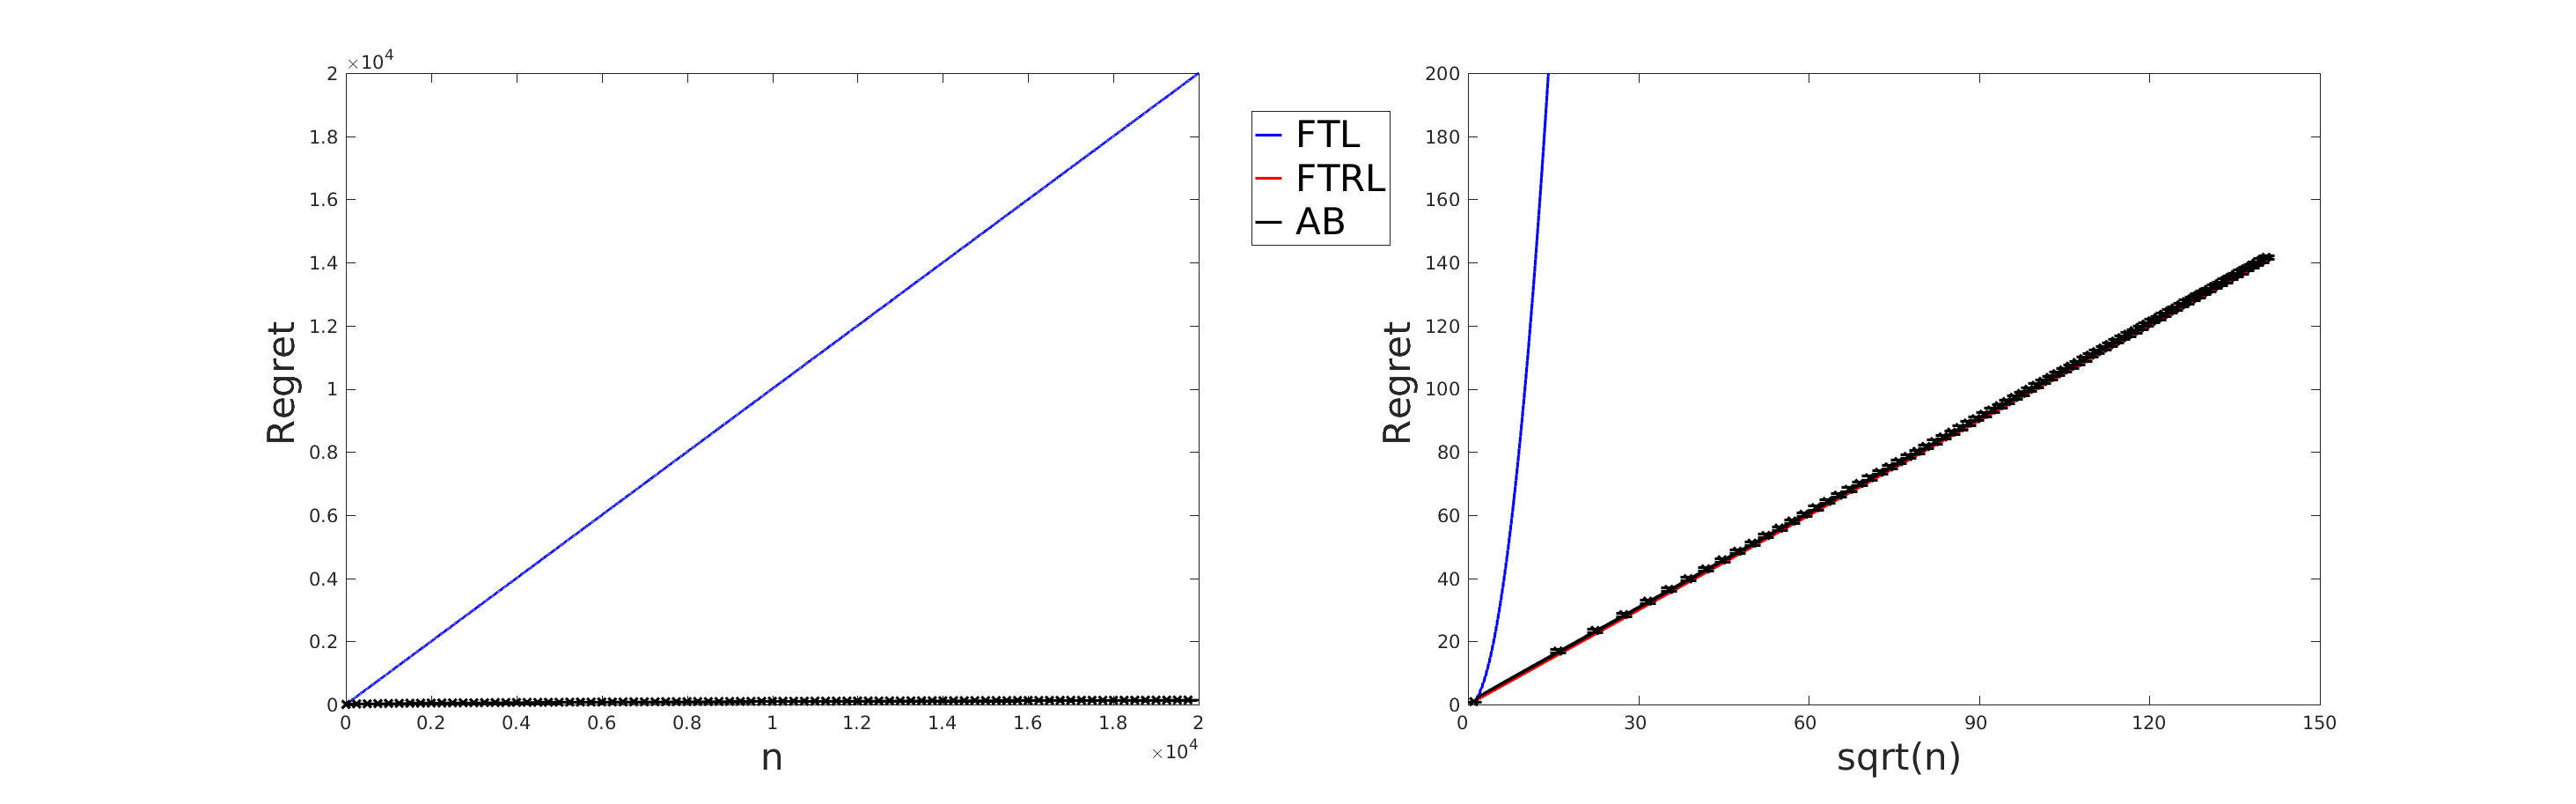
\includegraphics[width=0.8\textwidth]{figures/ExpResults/WorstCase_alt_new}
					\smallskip
					\footnotesize
					\begin{itemize}
						\item[-] $f_t=(\hf_t,0,0,0)$
						\item[-] $(\hf_t)_t = 0.9, -1,1,-1,1,\ldots$
					\end{itemize}
					\vspace{-1cm}	
				\end{block}				
			\end{minipage}
		\end{block}
		
		\vspace{0.0ex}
		\begin{block}{Conclusion}	
			\vspace{-0.3cm}
			\begin{itemize}
				\item[-] Shape of the constraint set may help. \medskip
				\item[-] Other algorithms? \medskip
				\item[-] Can the curvature of the constraint set help with curved loss functions?
				\vspace{-0.3cm}
			\end{itemize}
		\end{block}
		\vspace{0.0ex}
	\end{column}
		
	\begin{column}{0.01\textwidth}
	\end{column}
\end{columns}

\medskip

\begin{columns}
	\begin{column}{0.01\textwidth}
	\end{column}
	\begin{column}{0.98\textwidth}
		\begin{block}{References}
			\vspace{-0.1cm}
			\tiny
			\begin{center}
			\begin{minipage}{0.98\textwidth}
			\begin{multicols}{3}
			\bibliographystyle{plain}
			\bibliography{reference}
			\end{multicols}
			\end{minipage}
			\end{center}
			\vspace{-0.1cm}
		\end{block}
	\end{column}
	\begin{column}{0.01\textwidth}
	\end{column}	
\end{columns}		
 %\end{center}
\end{frame}

\end{document}
